\documentclass{article}

% if you need to pass options to natbib, use, e.g.:
% \PassOptionsToPackage{numbers, compress}{natbib}
% before loading nips_2017
%
% to avoid loading the natbib package, add option nonatbib:
% \usepackage[nonatbib]{nips_2017}

\usepackage[final]{nips_2017}
\PassOptionsToPackage{numbers}{natbib}

% to compile a camera-ready version, add the [final] option, e.g.:
% \usepackage[final]{nips_2017}
\usepackage[latin1]{inputenc} % allow utf-8 input
\usepackage[T1]{fontenc}    % use 8-bit T1 fonts
\usepackage{hyperref}       % hyperlinks
\usepackage{url}            % simple URL typesetting
\usepackage{booktabs}       % professional-quality tables
\usepackage{amsmath}
\usepackage{amsfonts}       % blackboard math symbols
\usepackage{nicefrac}       % compact symbols for 1/2, etc.
\usepackage{microtype}      % microtypography

\usepackage{dsfont}

\usepackage{algorithm}
\usepackage{algorithmic}

\usepackage{graphicx} 

\newcommand{\abs} [1] {\left| #1 \right|}
\newcommand{\norm}[1]{\left\|#1\right\|}
\newcommand{\scal}[2]{\langle #1,#2 \rangle}
\DeclareMathOperator{\R}{\mathbb{R}}
%\DeclareMathOperator{\det}{\mathrm{det}}

\title{Graph Sampling with Determiantal Point Processes}

\author{
	Quentin CHAN-WAI-NAM \\ MVA
	\And
	Guillaume GAUTIER (tutor) \\ INRIA
}
\date{08/01/2017}

\begin{document}

\maketitle

\begin{abstract}
	A great variety of data is originally structured as networks, or graphs. Data
	defined on the nodes of a given graph is called a graph signal. Here, we are
	interested in some results of the sampling theory, that state it is possible
	under some assumptions to reconstruct a graph signal given its values on only
	a node sample of size much smaller than the entire graph. We focus here on
	graph sampling using determinantal point processes, which are very useful
	tools to choose the nodes on which to sample the signal. This project is
	mainly focused on implementation and experimentation using results from \cite{tremblay2017}.
\end{abstract}


\section{Theory}


\subsection{Frequencies on graphs}


The goal of the sampling theory on graphs \cite{shuman2012} is similar to the goal of the Fourier sampling theory on classical signals: we try to decompose a given signal on some frequencies and use this decomposition to build a much compressed representation of the signal. Given a graph with $N$ nodes, we define the Laplacian matrix as:
\[ L = D - W \]
where $W \in \R^{N \times N}$ is the matrix of the edges of the graph such that $W_{i, j} \geq 0$ is the weight of the edge between nodes $i$ and $j$, and $D \in \R^{N \times N}$ is diagonal with $D_{i} = \sum_j W_{i, j}$. Let $(\Lambda, U)$ be the eigendecomposition of $L$ such that $\Lambda = (\lambda_1, \cdots, \lambda_N)^\top$, $0 = \lambda_1 \leq \cdots \leq \lambda_N$ and $U = (u_1, \cdots, u_N)$ are the associated eigenvectors. We say that $U_k = (u_1, \cdots, u_k)$ are the $k$ first low-frequency eigenmodes and any linear combination of $u_1, \cdots, u_k$ is called a $k$-bandlimited signal. Alternatively, $x$ is a $k$-bandlimited signal iff
\begin{align} \exists \; \alpha \in \R^k, \qquad x = U_k \alpha. \label{eq:bandlimited}\end{align}


\subsection{Sampling on graphs and signal reconstruction}


Sampling consists in choosing $m$ nodes among $N$ and measuring the signal on these nodes. If $\mathcal{A} = (\omega_1, \cdots, \omega_m)$ is the subset of the chosen nodes, $M \in R^{m \times N}$ is the measurement matrix such that $M_{i, j} = \delta_{j = \omega_i}$. Then a measurement of the signal $x$ on the sample $\mathcal{A}$ writes
\begin{align} y &= M x + \mathcal{N} \label{eq:measurement}\end{align}
where $\mathcal{N} \in \R^m$ is a measurement noise.


One can show that if $x$ is a $k$-bandlimited signal, then one can hope to reconstruct $x$ if $m \geq k$. The difficulty of the sampling theory is, given a measurement budget $m$, to find $\mathcal{A}$ such that $\abs{\mathcal{A}} = m$ and we can invert \eqref{eq:measurement} so as to reconstruct exactly $x$ from $y$. A sufficient condition for this to be true if $\mathcal{N} \equiv 0$ is that 
\begin{align} \text{$MU_k$ has its smallest singular value $\sigma_1 > 0$.} \label{eq:sufficientconditionreconstruction}\end{align}


\subsection{Reconstruction with determinantal point processes on graphs}


The \emph{determinantal point processes} (DPP) \cite{kuelsza2012} are tools that are very useful in this situation, since they enable to sample points in $\left\{ 1, \cdots, N\right\}$ with some negative correlation between the occurences of points that are ``close'' to each other, that is ``close'' points will be less likely to be sampled together. In other terms, sampling from a DPP ensures the diversity of the sample.


In our case, if $\left\{ 1, \cdots, N\right\}$ are the nodes of the graph, the random variable $\mathcal{A}$ from a DPP of \emph{marginal kernel} $K \in \R^{N \times N}$ verifies
\begin{align} \forall \mathcal{S} \subset \mathcal{A}, \qquad \mathbb{P}(\mathcal{S} \subset \mathcal{A}) = \det(K_\mathcal{S}) \label{eq:defDPP}\end{align}
where $K_\mathcal{S}$ is the submatrix of $K$ with lines and columns indices in $\mathcal{S}$.


When sampling the measurement nodes, if $x_1$ and $x_2$ are two graph signals, we want to ensure that $\norm{x_1 - x_2} > 0 \implies \norm{y_1 - y_2} > 0$. One way to ensure this is to reweight the measurement with a given matrix such that the norm of the reweighted measurement is close to the norm of the original vector. More specifically, if $\mathcal{A} = (\omega_1, \cdots, \omega_m)$, we define $P = \mathrm{diag}(\pi_{\omega_1}, \cdots, \pi_{\omega_m})$, and we have:
\begin{align} \mathbb{E}_\mathcal{A} \left( \norm{P^{-\frac{1}{2}} M x}^2 \right) = \norm{x}^2. \label{eq:esp_reweighted_norm}\end{align}
Thus, if we know the spanning eigenspace $U_k$, we can write the reconstruction problem as:
\begin{align*} x_{\text{rec}} &= \mathrm{argmin}_{z \in \mathrm{span}(U_k)} \norm{P^{-\frac{1}{2}} \left( M z - y \right)}^2 \\
&= U_k \; \mathrm{argmin}_{\alpha \in \R^m} \norm{P^{-\frac{1}{2}} \left( M U_k \alpha - y \right)}^2 \end{align*}
\begin{align} \boxed{x_\text{rec} = U_k (U_k^\top M^\top P^{-1} M U_k)^{-1} U_k^\top M^\top P^{-1} y}. \label{eq:reconstruction:dpp} \end{align}
In order to use the last formula, we must compute the inverse of an $N \times N$ matrix, which might be unfeasible if $N$ is large. One could then use other methods, such as gradient descent.


The next step is then to find some marginal kernel $K$ such that $x_\text{rec} = x$ with \eqref{eq:reconstruction:dpp}. We can show that if we use the kernel 
\begin{align} \boxed{K_k = U_k U_k^\top}, \label{eq:def:Kk}\end{align}
then any sample $\mathcal{A}$ from this DPP verifies $\abs{\mathcal{A}} = k$ a.s., \eqref{eq:sufficientconditionreconstruction} and thus perfect reconstruction can be achieved if there is no noise.


\subsection[Reconstruction with unknown Uk using DPPs]{Reconstruction with unknown $U_k$ using DPPs}


In the preceding sections, we assumed $U_k$ was known. It is possible, if $N$ is very large, that the computation of $U_k$ is unfeasible ; in this situation, we can not use the DPP given by $K_k$. A possible substitute is to consider the kernel:
\begin{align} \boxed{K_q = U g_q(\Lambda) U^\top} \label{eq:def:Kq}\end{align}
where $q > 0$ and $g_q(\lambda) = \frac{q}{q + \lambda}$. We can note that this is in fact an approximation of the kernel $K_k = U_k U_k^\top = U h_k(\Lambda) U^\top$ where $h_k(\lambda) = \mathds{1}_{\lambda \leq \lambda_k} (\lambda)$. Moreover, there exists an Algorithm that enables sampling from the DPP of marginal kernel $K_q$ without having to compute explicitely $K_q$, which makes this DPP particularly interesting.


In this case, we do not know explicitely $U_k$ so we can not use the direct reconstruction formula \eqref{eq:reconstruction:dpp}. Instead, we can use a regularized version of this formula that penalizes high frequencies:
\begin{align} \boxed{x_{\text{rec}} = \mathrm{argmin}_{z \in \R^N} \norm{P^{-\frac{1}{2}} \left( M z - y \right)}^2 + \gamma z^\top L^r z} \label{eq:reconstruction:dpp:unknown}\end{align}
where $\gamma > 0$, $r > 0$ are regularization parameters.

\section{Implementation details}


This project was mainly focused on implementation and experimentation. We used Python to implement the main algorithms. The code can be found here:
\begin{center}
  \url{https://github.com/14chanwa/graphsmlProject}
\end{center}


As we explained in the preceding section, our work decomposes in the following parts:
\begin{enumerate}
\item Generation of some graphs for benchmarking. We chose to work with community-structured graphs, as in \cite{tremblay2017}.
\item Generation of $k$-bandlimited signals as in \eqref{eq:bandlimited}.
\item Sampling DPPs with marginal kernel $K_k$ as in \eqref{eq:def:Kk}.
\item Sampling DPPs with marginal kernel $K_k$ as in \eqref{eq:def:Kq}.
\item Reconstruct $x$ from $y$ as in \eqref{eq:measurement} using the formula with known $U_k$ \eqref{eq:reconstruction:dpp}.
\item Reconstruct $x$ from $y$ as in \eqref{eq:measurement} using the formula without $U_k$ \eqref{eq:reconstruction:dpp:unknown}.
\end{enumerate}


Since $L$ and $W$ are sparse, we used functions from \verb#scipy.sparse# as much as possible, for our implementation to scale well with $N$.


\subsection{Random graph generation} \label{subs:random_graph_generation}


\paragraph{Function} \verb#generate_graph_from_stochastic_block_model#


For benchmarks, we chose to use community-structured graphs using the Stochastic Block Model (SBM) as in \cite{tremblay2017}. Consider a graph with $k$ communities of cardinal $N/k$. An edge has a probability $q_1$ to be drawn between nodes $i$ and $j$ if they belong to the same community, and $q_2$ else. We can then parameterize the SBM with $N, k, q_1, q_2$, or alternatively with $N, k, \epsilon, c$ where $\epsilon = \frac{q_2}{q_1}$ and $c = q_1 \left( \frac{N}{k} - 1 \right) + q_2 \left(N - \frac{N}{k}\right)$ is the average degree of a node in the graph. One can also show that there is a critical value of $\epsilon$, $\epsilon_c = (c - \sqrt{c})/(c + \sqrt{c}(k-1))$ above which the community structure becomes undetectable for large $N$'s, so we can also use the ratio $\epsilon/\epsilon_c$ as a parameter.


We used the Python library NetworkX \cite{hagberg2008} to generate $L$, $W$ and provide the necessary plot functions. 


\subsection[Generation of k-bandlimited signals]{Generation of $k$-bandlimited signals} \label{subsec:gen:k:bandlimited}


\paragraph{Function} \verb#generate_k_bandlimited_signal#


In order to generate a $k$-bandlimited signal, we must compute $U_k$ and take a linear combination of these vectors as in \eqref{eq:bandlimited}. This is equivalent to compute the $k$ lowest eigenmodes of the Laplacian matrix $L$. Even though we could use the function \verb#numpy.linalg.eigh# directly, we chose to use functions that scale better with $N$. The function \verb#scipy.sparse.eigh# uses a routine that enables to compute some eigenmodes from a sparse matrix. It is more efficient to compute the largest eigenmodes than the lowest ; we make use of the \emph{shift-inverse} mode\footnote{See: \url{https://docs.scipy.org/doc/scipy/reference/tutorial/arpack.html}} of this function in order to compute the lowest eigenmodes of $L$ by computing the largest eigenmodes of a dual problem.


\subsection[Sampling DPPs with marginal kernel Kk]{Sampling DPPs with marginal kernel $K_k$}


\paragraph{Function} \verb#sample_from_DPP#


We suppose $U_k$ known ; then we can compute $K_k = U_k U_k^\top$. We then have to build an algorithm that samples a DPP from a given marginal kernel $K$ ; we used the algorithm given in \cite{tremblay2017, kuelsza2012} in order to do so. 


Our version of this algorithm is presented in Algorithm \ref{alg:sampling_dpp_from_kernel}. Its principle is, given the eigendecomposition of $K$, to first sample some of its eigenvectors with probabilities given by their corresponding eigenvalues. Then, we select recursively the nodes of the sample with probabilities given by the selected eigenvectors.


\begin{algorithm}[ht]
\caption{Sampling a DPP with marginal kernel $K$}
\label{alg:sampling_dpp_from_kernel}
\begin{algorithmic} % enter the algorithmic environment
    \STATE \textbf{Input:} Eigendecomposition of $K$: $(\Lambda, V)$
    \STATE $J \leftarrow \emptyset$
		\FOR{$n = 1..N$}
			\STATE $J \leftarrow J \cup \left\{ n \right\}$ with probability $\lambda_n$
		\ENDFOR
		\STATE $V \leftarrow \left\{ v_n \right\}_{n \in J}$
		\STATE $Y \leftarrow \emptyset$
    \WHILE{$\abs{V} > 0$}
        \STATE $P \leftarrow (\norm{v_i}^2)_{i=1..\abs{V}}^\top / \abs{V}$ (vector of size $N$)
				\STATE $i \leftarrow$ choice of $i$ in $1..N$ with probability $P$
				\STATE $Y \leftarrow Y \cup \left\{i\right\}$
				\IF{$\abs{V} > 1$}
					\STATE $j \leftarrow$ index of a $v_j$ such that $\scal{v_j}{e_i} \neq 0$.
					\STATE Remove a linear combination of $v_j$ from $v_{j'}, j'\neq j$ such that $\forall j', \; \scal{v_{j'}}{e_i} = 0$.
					\STATE Delete $v_j$ from $V$.
					\STATE Use Gram-Schmidt algorithm to orthonormalize $V$.
				\ELSE
					\STATE \textbf{break}
				\ENDIF
    \ENDWHILE
		\STATE \textbf{Return:} $Y$
\end{algorithmic}
\end{algorithm}



In order to use this algorithm on $K_k$, we must be able to compute at least the $k$ first eigenmodes of $K_k$ (since the other eigenvalues of $K_k$ are null, we do not make use of the corresponding eigenmodes) ; we could use the same technique as in Subsection \ref{subsec:gen:k:bandlimited}.%, but in order to keep the algorithm generic, we chose to use the regular function \verb#numpy.linalg.eigh# in this case.


\subsection[Sampling DPPs with marginal kernel Kq (Wilson's algorithm)]{Sampling DPPs with marginal kernel $K_q$ (Wilson's algorithm)}


\paragraph{Functions} \verb#wilson_algorithm#, \verb#generate_maze#
\paragraph{Test file} \verb#test_generate_maze.py#


This is the main contribution of \cite{tremblay2017} ; in order to avoid computing $K_k$ (and thus $U_k$), the author uses an approximation $K_q$ and gives an algorithm capable of sampling from the DPP of marginal kernel $K_q$ without explicitely computing the kernel. This algorithm is based on a modified version of Propp-Wilson's algorithm \cite{propp1998}. 


Originally, this algorithm samples a random spanning tree of a given directed graph. A recreational application of this algorithm is random maze generation: consider a graph composed of nodes on a grid, plus a node that will represent the border of the maze. The walls will be lines connecting these nodes: consider then the appropriate edges of this graph (two nodes are connected if they are adjacent, the border node is connected to all nodes in the border). Then when sampling a random spanning tree on this graph, one samples the walls of a maze such that there is one and only one way from one corridor to the other that do not imply turning back. We implemented this random maze generation in order to make sure our algorithm works, as presented in Figure \ref{fig:randommazes}.


\begin{figure}[ht]
\centering
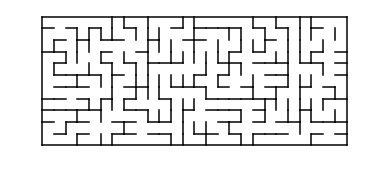
\includegraphics[height=3cm]{maze1.png}
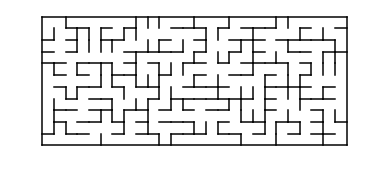
\includegraphics[height=3cm]{maze2.png}
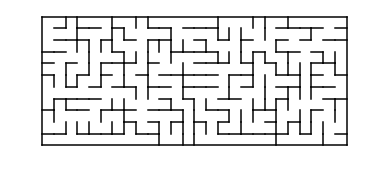
\includegraphics[height=3cm]{maze3.png}
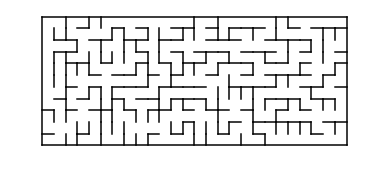
\includegraphics[height=3cm]{maze4.png}
\caption{Examples of random mazes generated with random spanning trees on a grid of $25\times10$ wall nodes plus the border node.}\label{fig:randommazes}
\end{figure}


The original algorithm works using loop-erased random walks in the graph until all nodes have been visited. In \cite{tremblay2017}, we modify the algorithm so that it samples nodes from the graph by adding a sink node. At each step of the random walks, the walker has some probability depending on a parameter $q$ to go to the sink: the last visited node is then part of the sample. This algorithm is presented in Algorithm \ref{alg:wilson_algorithm}.


\begin{algorithm}[ht]
\caption{Wilson's algorithm}
\label{alg:wilson_algorithm}
\begin{algorithmic} % enter the algorithmic environment
    \STATE \textbf{Input:} Adjacency matrix $W$, sink weight $q \geq 0$
    \STATE $Y, \nu \leftarrow \emptyset$
		\WHILE{$\nu \neq \left\{1, \cdots, N\right\}$}
			\STATE Begin a random walk $S$ from a node $i \notin \nu$.
			\IF{it reaches itself} 
				\STATE Erase the loop in the walk.
			\ELSIF{it reaches some node in $\nu$ or the sink $\Delta$}
				\STATE $\nu \leftarrow \nu \cup S$
				\IF{the last node is $\Delta$}
					\STATE If $\ell$ is the last visited node before $\Delta$, then $Y \leftarrow Y \cup \left\{\ell\right\}$.
				\ENDIF
			\ENDIF
		\ENDWHILE
		\STATE \textbf{Return:} $Y$
\end{algorithmic}
Note: our implementation also saves the sampled spanning tree. In the case $q = 0$, there is no sink and we have the original Propp-Wilson algorithm.
\end{algorithm}


\section{Results}


\subsection[Sampling from Kk]{Sampling from $K_k$}


\paragraph{Test file} \verb#test_sample_from_Kk.py#


In order to make sure we sample the right DPP with marginal kernel $K_k$ with our Algorithm \ref{alg:sampling_dpp_from_kernel}, we generate a graph from the SBM (as in Subsection \ref{subs:random_graph_generation}) and sample from our algorithm a number of times $n$. If the algorithm is correct:
\begin{itemize}
\item Every sample is of size $k$ (this is verified in practice).
\item For any singleton $i$, $p(i \in \mathcal{A}) = K_{i, i}$ \eqref{eq:defDPP}.
\item For any pair $i, j$, $i < j$, $p(i \in \mathcal{A} $ and $ j \in \mathcal{A}) = \det \begin{pmatrix} K_{i, i} & K_{i, j} \\ K_{j, i} & K_{j, j} \end{pmatrix}$ \eqref{eq:defDPP}.
\item For a given $k$-bandlimited signal $x$, $\mathbb{E}_\mathcal{A} \left( \norm{P^{-\frac{1}{2}} M x}^2 \right) = \norm{x}^2$ \eqref{eq:esp_reweighted_norm}.
\end{itemize}


We choose two singletons and two pairs, and we compute the empirical probabilities and expectations over the $n=50000$ samples, with $N=100$, $k=2$, $c=16$, $\epsilon = 0.5 \times \epsilon_c$. The results are presented in Table \ref{tab:Kk:verification}.


\begin{table}[th]
  \caption{Verification of the correctness of the sampling algorithm for $K_k$.}
  \label{tab:Kk:verification}
  \centering
  \begin{tabular}{lll}
    \toprule
    Test &  Theoretical proba & Empirical proba \\
    \midrule
    Singleton 1 & $0.01895$ & $0.01824$ \\
    Singleton 2 & $0.01078$ & $0.01006$ \\
    Pair 1 & $0.00015$ & $0.00016$ \\
		Pair 2 & $0.00025$ & $0.00020$ \\
    \bottomrule
  \end{tabular}
	\quad
	\begin{tabular}{lll}
    \toprule
    Test &  $\norm{x}_2^2$ & $\norm{P^{-1/2} M x}_2^2$ \\
    \midrule
    Norm & $1.0$ & $1.00074$ \\
    \bottomrule
  \end{tabular}
\end{table}

%\begin{verbatim}
%TODO: make a table instead
%------- Singleton:
%Theoretical proba= 0.0189521762207
%Empirical proba= 0.01824
%------- Singleton2:
%Theoretical proba= 0.010781904604
%Empirical proba= 0.01006
%------- Pair:
%Theoretical proba= 0.000152315628169
%Empirical proba= 0.00016
%------- Pair2:
%Theoretical proba= 0.000256030200653
%Empirical proba= 0.0002
%------- Norms:
%mean np.linalg.norm(x)**2= 1.0
%mean np.linalg.norm(Pm12.dot(M).dot(x))**2= 1.00074165703
%\end{verbatim}


We thus confirm that our algorithm samples the right DPP.


\subsection[Sampling from Kq]{Sampling from $K_q$}


\paragraph{Test file} \verb#test_sample_from_Kq.py#


We proceed the same way with our Algorithm \ref{alg:wilson_algorithm} that samples from a DPP with marginal kernel $K_q$, with the difference that the size of the sample is not fixed. Rather, we should have:
\begin{align} \mathbb{E}\left( \abs{\mathcal{A}}\right) = \sum_{i=1}^{N} \frac{q}{q+\lambda_i}. \end{align}


Since this sampling algorithm is much slower than the preceding one, we chose to test the following parameters: $n=10000$ samples, with $N=100$, $k=2$, $c=16$, $\epsilon = 0.5 \times \epsilon_c$ and $q=1.0$. The results are presented in Table \ref{tab:Kq:verification}.

\begin{table}[th]
  \caption{Verification of the correctness of the sampling algorithm for $K_q$.}
  \label{tab:Kq:verification}
  \centering
  \begin{tabular}{lll}
    \toprule
    Test &  Theoretical proba & Empirical proba \\
    \midrule
    Singleton 1 & $0.06752$ & $0.06570$ \\
    Singleton 2 & $0.05920$ & $0.05590$ \\
    Pair 1 & $0.00418$ & $0.00450$ \\
		Pair 2 & $0.00470$ & $0.00490$ \\
    \bottomrule
  \end{tabular}
	\quad
	\begin{tabular}{lll}
    \toprule
    Test &  $\norm{x}_2^2$ & $\norm{P^{-1/2} M x}_2^2$ \\
    \midrule
    Norm & $1.0$ & $1.00290$ \\
    \bottomrule
  \end{tabular} \\
	\vspace{0.5cm}
	\begin{tabular}{lll}
    \toprule
    Test &  Theoretical & Empirical \\
    \midrule
    Cardinal & 6.95801 & 6.96870 \\
    \bottomrule
  \end{tabular}
\end{table}
		
%\begin{verbatim}
%TODO: make a table instead
%------- Cardinal
%Theoretical= 6.95800812053
%Empirical= 6.9687
%------- Singleton:
%Theoretical proba= 0.067520041977
%Empirical proba= 0.0657
%------- Singleton2:
%Theoretical proba= 0.059207968264
%Empirical proba= 0.0559
%------- Pair:
%Theoretical proba= 0.00417738808421
%Empirical proba= 0.0045
%------- Pair2:
%Theoretical proba= 0.0047052228183
%Empirical proba= 0.0049
%------- Norms:
%mean np.linalg.norm(x)**2= 1.0
%mean np.linalg.norm(Pm12.dot(M).dot(x))**2= 1.00289718132
%\end{verbatim}

We thus confirm that our algorithm samples the right DPP.

\subsection[Signal reconstruction with Kk qnd known Uk]{Signal reconstruction with $K_k$ and known $U_k$}


\paragraph{Test file} \verb#test_recovery_with_Kk.py#


In the following we choose $N=100$, $k=2$, $c=16$, $\epsilon = 0.1 \times \epsilon_c$. We use the DPP of marginal kernel $K_k$ to sample $k$ measurement nodes, compute exactly $P$ by using the diagonal of $K_k$ and use the perfect reconstruction formula \eqref{eq:reconstruction:dpp}. The article presents the influence of $\epsilon$ on the reconstruction error ; we chose to compute the influence of the noise standard deviation $\sigma$ of the noise $\mathcal{N}$ on the reconstruction error, where
\[ y = Mx + \mathcal{N}. \] 
We generate $100$ graphs using the preceding parameters, and on each graph we generate $100$ $k$-bandlimited signals. On each graph, we sample $k$ measurement nodes and on each signal, we add $\mathcal{N}$ with a given $\sigma$. We then compute the reconstruction error.


When $\mathcal{N} \equiv 0$, our algorithm reconstructs the signal perfectly, up to the machine precision (the mean error is $\sim 10^{-15}$, the max error is $\sim 10^{-8}$). When we increase $\sigma$, the reconstruction error increases. The results are presented in Figure \ref{fig:Kk:recerror}.


\begin{figure}[ht]
\centering
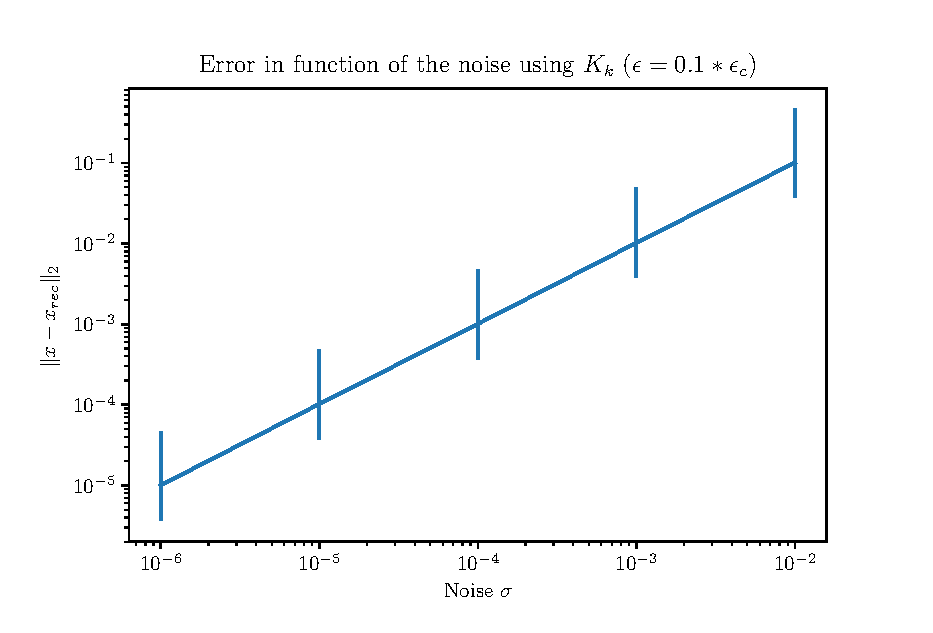
\includegraphics[height=8cm]{error_function_noise_Kk.eps}
\caption{Influence of $\sigma$ on the reconstruction error (DPP of marginal kernel $K_k$, reconstruction using \eqref{eq:reconstruction:dpp}). The error bars are the $10^\text{th}$ and $90^\text{th}$ percentiles.} \label{fig:Kk:recerror}
\end{figure}


We note that there are rare cases in which our reconstruction algorithm fails spectacularly. The max reconstruction errors are presented in Table \ref{tab:Kk:maxrecerror}. 


\begin{table}[ht]
  \caption{Max reconstruction error (DPP of marginal kernel $K_k$, reconstruction using \eqref{eq:reconstruction:dpp})}
  \label{tab:Kk:maxrecerror}
  \centering
  \begin{tabular}{ll}
    \toprule
    Noise $\sigma$ &  Max reconstruction error \\
    \midrule
    $10^{-6}$ & $0.16$ \\
    $10^{-5}$ & $1.46$ \\
    $10^{-4}$ & $5.88$ \\
		$10^{-3}$ & $64$ \\
		$10^{-2}$ & $675$ \\
    \bottomrule
  \end{tabular}
\end{table}


%TODO: when no noise, perfect reconstruction ; when noise, sometimes it fails spectacularly, most of the time the error norm is small (10, 50, 90 quantiles)


\subsection[Signal reconstruction with Kq and known Uk]{Signal reconstruction with $K_q$ and known $U_k$}


\paragraph{Test file} \verb#test_recovery_with_Kq.py#


In this section, we still assume $U_k$ is known. The kernel $K_q$ is build so as to be an approximation of $K_k$. This enables us to sample from $K_q$ without having to explicitely compute $K_q$. We thus try to use the sampling algorithm with $K_q$ to choose the measurement nodes and reconstruct the signal using \eqref{eq:reconstruction:dpp} just as in the preceding section. We use the parameters $N=100$, $k=2$, $c=16$, $\epsilon = 0.1 \times \epsilon_c$ and sample 100 graphs and 100 signals on each graph, then add the corresponding noise levels.


We can not set a specific cardinal for the samples of our DPP with kernel $K_q$ ; it depends on a parameter $q$. We chose to fix and initial $q_\text{init}=0.2$ and increase $q$ if the sample is of size $m < k$ with the algorithm suggested in the article. In our tests, the mean cardinal of our sample is $3.11$. 


The results are presented in Figure \ref{fig:Kq:recerror}. We see that the reconstruction noise is comparable to the algorithm sampling from $K_k$. This means that $K_q$ is effectively a good approximation of $K_k$. We could argue that this comparison might be unfair since the mean cardinal of our sample is $3.11 > k = 2$ ; yet the algorithm $K_k$ can not produce samples of size $\neq k$, whereas in Wilson's algorithm we can set the expected sample size with the parameter $q$, that makes this algorithm more adaptable. 


Similarly, there are cases in which the algorithm fails spectacularly, as presented in Table \ref{tab:Kq:maxrecerror}.


\begin{figure}[ht]
\centering
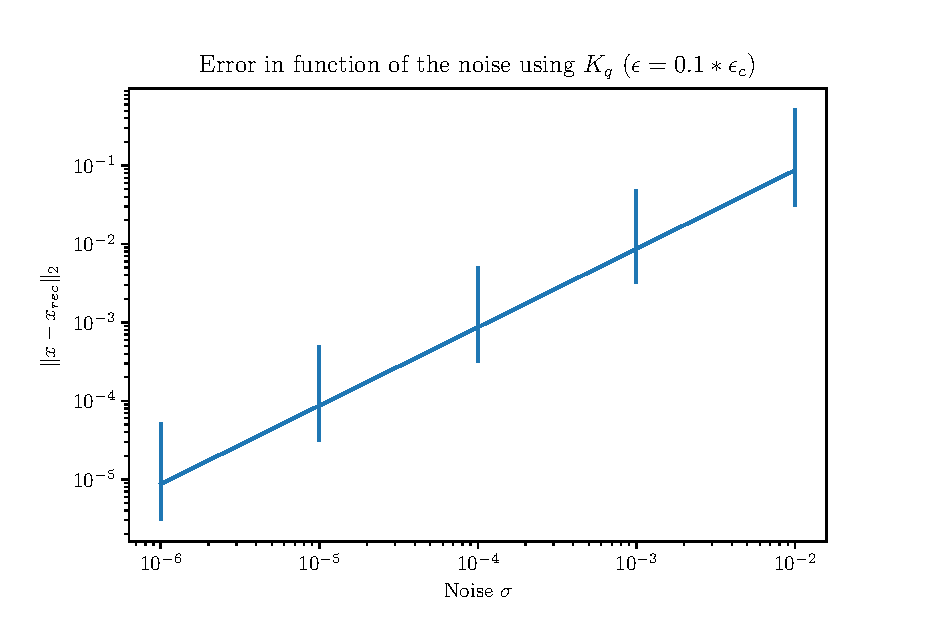
\includegraphics[height=8cm]{error_function_noise_Kq.eps}
\caption{Influence of $\sigma$ on the reconstruction error (DPP of marginal kernel $K_q$, reconstruction using \eqref{eq:reconstruction:dpp}). The error bars are the $10^\text{th}$ and $90^\text{th}$ percentiles.} \label{fig:Kq:recerror}
\end{figure}


\begin{table}[ht]
  \caption{Max reconstruction error (DPP of marginal kernel $K_q$, reconstruction using \eqref{eq:reconstruction:dpp})}
  \label{tab:Kq:maxrecerror}
  \centering
  \begin{tabular}{ll}
    \toprule
    Noise $\sigma$ &  Max reconstruction error \\
    \midrule
    $10^{-6}$ & $0.06$ \\
    $10^{-5}$ & $1.56$ \\
    $10^{-4}$ & $12.9$ \\
		$10^{-3}$ & $187$ \\
		$10^{-2}$ & $1091$ \\
    \bottomrule
  \end{tabular}
\end{table}


\subsection[Signal reconstruction with Kq and unknown Uk]{Signal reconstruction with $K_q$ and unknown $U_k$}


For now, we only used \eqref{eq:reconstruction:dpp}, which requires the knowledge of $P = \mathrm{diag} (\pi_{\omega_1}, \cdots, \pi_{\omega_1})$ and $U_k$. Yet in order to compute $P$, one has to compute the marginal kernel associated to the DPP used to sample the nodes and $U_k$. This is exactly what we wanted to avoid in the first place.


TODO: regularization not working yet

	
\newpage
\bibliography{bibliography} 
\bibliographystyle{plain}

\end{document}
